\begin{figure}[h]
\centering
\begin{tikzpicture}
\node [anchor=west] (scope) at (8.75,5.5) {Embodied Costs};
\node [anchor=west] (traffic) at (1.4,5.5) {Traffic};
\node [anchor=west] (bem) at (4.2,5.5) {BEM};
\node [anchor=west] (mec) at (6.75,5.5) {MEC};
\begin{scope}[xshift=1.5cm]
    \node[anchor=south west,inner sep=0] (image) at (0,0) {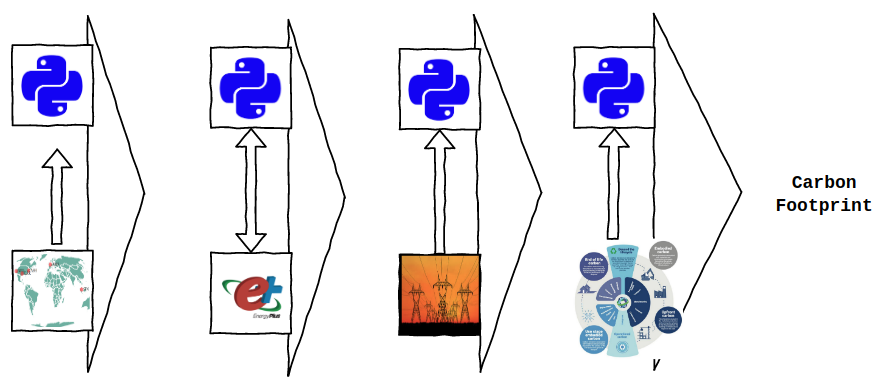
\includegraphics[width=0.8\textwidth]{embodied_cost_model/images/horizontal_process_flow.png}};
    \begin{scope}[x={(image.south east)},y={(image.north west)}]
        % \draw[ultra thick,rounded corners, ,dashed] (0.625,1.0) rectangle (0.85,0.0);
        % \draw [-stealth, line width=5pt, cyan] (scope) -- ++(0.6,0.0);
    \end{scope}
\end{scope}
\end{tikzpicture}
\caption[Model Process Flow Diagram]{Model Process Flow Diagram.}
\label{process_flow}
\end{figure}